\documentclass{article}
\usepackage{amsfonts}
\usepackage{amsthm}
\usepackage{amssymb}
\usepackage{amsmath}
\usepackage{graphicx}
\usepackage{subcaption}
\usepackage{xcolor}
\usepackage{mathtools}
\usepackage{ wasysym }
\usepackage{enumerate}
\usepackage{verbatim}


\numberwithin{equation}{section}
\newcommand{\new}[2]{
    \vspace{2mm}
    \noindent
    \textbf{
    \underline{#1}}
    \textit{{#2}}
    \
}

\def\<{{\langle}}
\def\>{{\rangle}}

\DeclarePairedDelimiter\bra{\langle}{\rvert}
\DeclarePairedDelimiter\ket{\lvert}{\rangle}
\DeclarePairedDelimiterX\braket[2]{\langle}{\rangle}{#1\,\delimsize\vert\,\mathopen{}#2}


\newcommand{\textOr}{
    {
        \hspace{5mm}
        \textrm{or}
        \hspace{5mm}
    }
}

\newcommand{\textAnd}{
    {
        \hspace{5mm}
        \textrm{and}
        \hspace{5mm}
    }
}


\newcommand{\textWhere}{
    {
        \hspace{5mm}
        \textrm{where}
        \hspace{5mm}
    }
}



\newcommand{\Ixp}[1]{
    {
        e^{i{#1}}
    }
}



\newcommand{\halfFigure}[1]{
\begin{center}
\includegraphics[width = .5\linewidth]{{#1}}
\end{center}
}

\newcommand{\fullFigure}[1]{
\begin{center}
\includegraphics[width = .9\linewidth]{{#1}}
\end{center}
}

\def\twobytwoMat(#1, #2, #3, #4){
    {
        \begin{bmatrix}
            {#1} & {#2}\\
            {#3} & {#4}
        \end{bmatrix}
    }
}

\def\twobyoneMat(#1, #2){
    {
        \begin{bmatrix}
            {#1}\\
            {#2}
        \end{bmatrix}
    }
}

\def\twobytwoDet(#1, #2, #3, #4){
    {
        \begin{vmatrix}
            {#1} & {#2}\\
            {#3} & {#4}
        \end{vmatrix}
    }
}


\newcommand{\deriv}[2]{
\frac {d {#1} } {d {#2}}
}

\newcommand{\dderiv}[2]{
\frac {d^2 {#1} } {d{#2}^2}
}

\newcommand{\pderiv}[2]{
\frac {\partial {#1} } {\partial {#2}}
}


\newcommand{\RR}{\mathbb{R}}
\newcommand{\CC}{\mathbb{C}}
\newcommand{\ZZ}{\mathbb{Z}}
\newcommand{\Zpos}{\mathbb{Z}_{pos}}
\newcommand{\NN}{\mathbb{N}}

\newtheorem{theorem}{Theorem} [section]
\newtheorem{proposition}{Proposition}[section]
\newtheorem{lemma}{Lemma}[section]
\newtheorem{corollary}{Corollary}[section]
\newtheorem{remark}{Remark}[section]
\newtheorem{definition}{Definition}[section]
\newtheorem{example}{Example}[section]
\newtheorem{conjecture}{Conjecture}[section]
\newtheorem{question}{Question}[section]

\newcommand{\ch}{\text{ch}}

\begin{document}
\begin{center}
    \Large
    \textbf{Lab 4 writeup, Numerical SE}

    \large
    Daniel Son
\end{center}

\section{Pre-Lab exercises}

\begin{question}
Solve the two differential equations under 
the initial conditions $(x(0), x'(0)) = (x_0, v_0)$. 
\begin{align}\label{eqn:diffeqs}
    \dderiv{x}{t} & = \ \lambda^2 x \\ 
    \dderiv{x}{t} & = \ -\omega^2 x 
\end{align}
\end{question}

\begin{proof}[Solution]
    Start with the first equation. The solution is some sum 
    of regular exponentials. We express the solution 
    as a sum of hyberbolic sin and cosine. 
    \begin{align}
        x \ = \ A \cosh(\lambda t) + B \sinh(\lambda t)
    \end{align}
    Imposing the initial condition $x(0) = x_0, x'(0) = v_0$, we 
    obatin the following solution. 
    \begin{align}
        x \ = \ x_0 \cosh(\lambda t) + v_0 \sinh(\lambda t)
    \end{align}

    The solution for the second equation is similar. Change the 
    hyperbolic trig functions to regular trig functions. 

\begin{align}
        x \ = \ A \cos(\lambda t) + B \sin(\lambda t)
    \end{align}
    Imposing the initial condition $x(0) = x_0, x'(0) = v_0$, we 
    obatin the following solution. 
    \begin{align}
        x \ = \ x_0 \cos(\lambda t) + v_0 \sin(\lambda t)
    \end{align}
\end{proof}

\begin{question}
    Consider a finite potential where the particle is 
    bounded, i.e. $E < V_0$. What is the decay constant 
    of the wavefunction of the particle outside the well? 
    Also, what is the wavelength of the particle within the 
    region?
\end{question}

\begin{proposition}
    Let $k$ be the decay constant and $\lambda$ the 
    wavelength. 
    \begin{align}
        k & = \ \frac{\sqrt{2m(V_0 - E)}}{\hbar} \\ 
        \lambda & = \  \frac{2 \pi \hbar}{\sqrt{2 m E}}
    \end{align}
\end{proposition}

\begin{proof} 
    Solve the TISE. 
    \begin{align}
        E \psi(x) \ = \ -\frac {\hbar^2}{2m} \psi''(x) + V(x) \psi(x)
    \end{align}
    Assuming $V(x)$ is constant around the region, the 
    equation simplifes to \eqref{eqn:diffeqs}. 
    \begin{align}
        (E - V(x)) \psi(x) \ = \ -\frac{\hbar^2}{2m} \psi''(x)
    \end{align}
    Within the well, the potential is zero. The solution is 
    an harmonic oscillator. Following Robinett's notation, 
    we label the wavenumber as $q$. 
    \begin{align}
        q \ = \ \frac {\sqrt{2mE}}{\hbar}
    \end{align}
    From the wavenumber, we derive the wavelength. 
    \begin{align}
        \lambda \ = \ \frac {2\pi} q \ = \ \frac{2 \pi \hbar}{\sqrt{2 m E}}
    \end{align}

    Outside the well, the potential has a value of $V_0$. Thus, 
    the decay constant is 
    \begin{align}
        k \ = \ \frac{\sqrt{2m(V_0 - E)}}{\hbar}. 
    \end{align}
\end{proof}

\begin{question}
Take a moment to work out the scaled TISE, or reference past work you may have done on a problem set. We’ll define an energy scale $E_0$ and a length scale $x_0$ and re-write the equation in terms of a dimensionless position $s = x / x_0$, energy $e = E / E_0$, and potential energy $v = V(x) / E_0$. If you do so, you should find that you can write the TISE in the form
\begin{equation}\label{eqn:dimensionless}
    \frac{d^2 \psi}{ds^2} = A (v(s) - e) \psi,
\end{equation}
where $A$ is a dimensionless constant. 

Find $A$ in terms of characteristic quantities, and then calculate its numerical value assuming that $x_0 = 1 \, \text{nm}$, $m = m_e$, and $E_0 = 1 \, \text{eV}$. You should find that for these parameters $A \approx 26.24$.
\end{question}


\begin{proof}[Solution]
    Faithfully applying the substitutions, 
    we find the following 
    formula for $A$. 
    \begin{align}
        A \ = \ 
        \frac {2m E_0 x_0 ^2 }{\hbar^2} 
        \ \approx \ 26.24
    \end{align}
\end{proof}

\begin{question}

Suppose that $V(x) = \frac{1}{2} m \omega^2 x^2$, as with a simple harmonic oscillator. Show that in this case we can write the TISE in the form
\[
    \frac{d^2 \psi}{ds^2} = A \left( \frac{1}{2} B s^2 - e \right) \psi,
\]
and find the constant $B$. You should see that for a suitable choice of scales $x_0$ and $E_0$ you can set both constants $A$ and $B$ to 1, allowing us to write the scaled TISE simply as
\[
    \frac{d^2 \psi}{ds^2} = \left( \frac{1}{2} s^2 - e \right) \psi.
\]
\end{question}

\begin{proof}
    It is straightforward to see that \begin{align}
        B \ = \ \frac {m \omega^2} {E_0}.
    \end{align}

    From \eqref{eqn:dimensionless}, we purport that a 
    subsitution $s = kl$ will simplify the equation into 
    the desired form. Rewriting the equation in terms of $l$, 
    we obtain the following. 
    \begin{align}
        \psi''(l) \ = \ k^2 A \left(
            \frac 1 2 B (kl)^2 - e 
        \right)\psi(l)
    \end{align}

    We wish 
    \begin{align}
        k^2 A  \ = \ 1 \textAnd k^4 A B \ = 1
    \end{align}
    which implies 
    \begin{align}
        k^2 B \ = \ 1 \textAnd A/B \ = \ 1
    \end{align}
    and imposing $A/B = 1$, we derive an expression 
    for the characteristic length with respect to the energy scale. 
    \begin{align}\boxed{
        x_0 \ = \ \frac {E_0} {\sqrt 2 \hbar}}
    \end{align}
\end{proof}


\section{FSW with barriers}
\subsection{Solution for the wavefunction with barrier}
Define our barrier potential to have width of 1, well 
height of $10V$, and barrier height of $5V$. 
\begin{figure}[h]
    \centering
    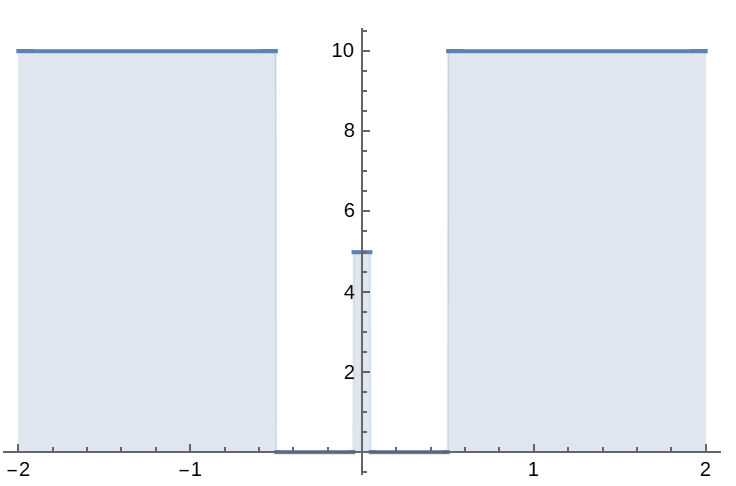
\includegraphics[width=0.4\textwidth]{III2_barrier.png} % Replace 'figure.jpg' with your image file
    \caption{Figure of the FSW with Barrier Potential}
    \label{fig:III_barrief}
\end{figure}

We first verify that there exists a case where 
the classical interpretation is violated. If 
the energy of the particle is less than the barrier potential 
of $5V$, then a particle confined in one side of the well 
should stay confined and not 'spill' to the neighboring well. 

\begin{figure}[h]
    \centering
    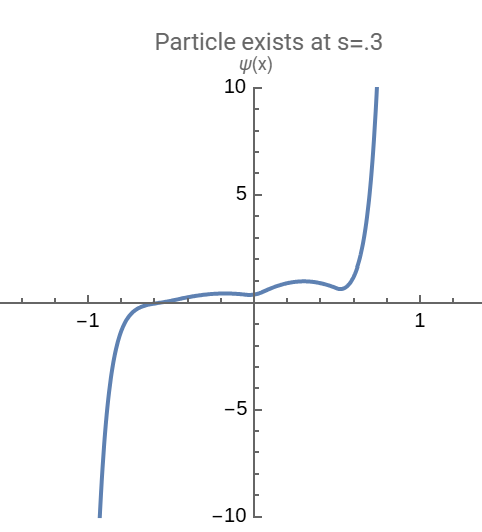
\includegraphics[width=0.4\textwidth]{III2_spill.png} % Replace 'figure.jpg' with your image file
    \caption{$E = 1, \psi(.3) = 1, \psi'(.3) = 0$. Apparently, the particle 
    has spilled over the well.}
    \label{fig:III_spill}
\end{figure}

\begin{figure}[h]
    \centering
    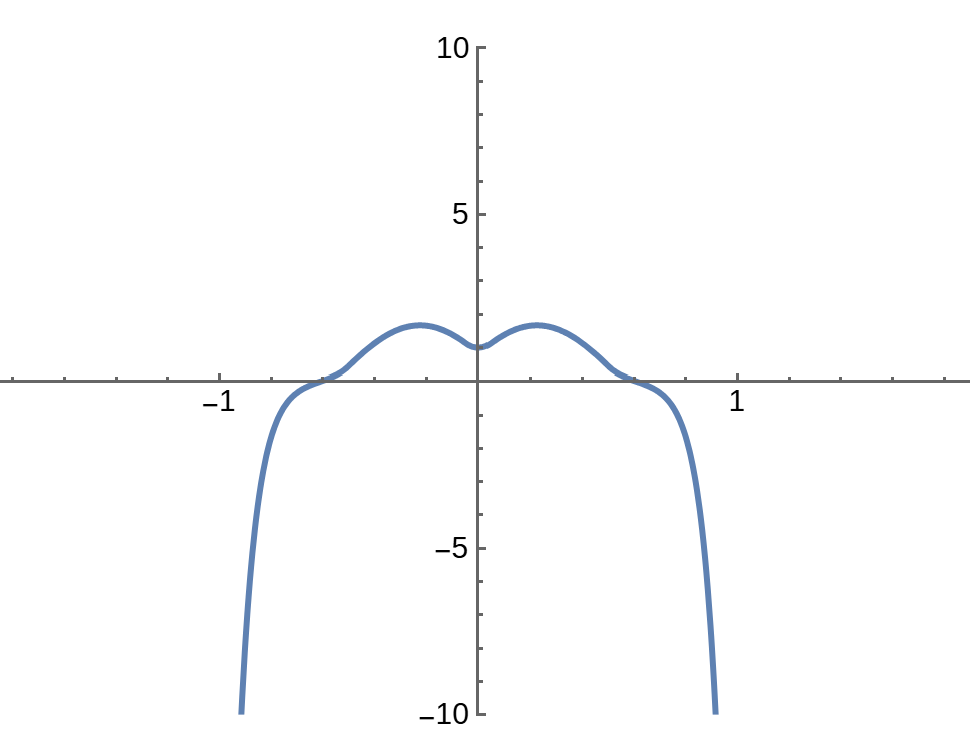
\includegraphics[width=0.8\textwidth]{III2_dimple.png} % Replace 'figure.jpg' with your image file
    \caption{Wavefunction of the lowest energy eigenstate. 
    Notice the 'dimple' on $s = 0$. }
    \label{fig:example}
\end{figure}


We also list out the first four energy eigenstates. 
\begin{align}
    E_1 \ = \ .83 && E_3 \ = \ 3.45 \nonumber\\ 
    E_2 \ = \ 1.21 && E_4 \ = \ 4.73
\end{align}


\textcolor{green}{Comparison with the FSW to be added}

\subsection{Taller and Wider Wells}

In this section, we investigate potentials 
that have varying barrier dimensions. 

\begin{figure}[htp]
    \centering
    \begin{subfigure}[b]{0.45\textwidth}
        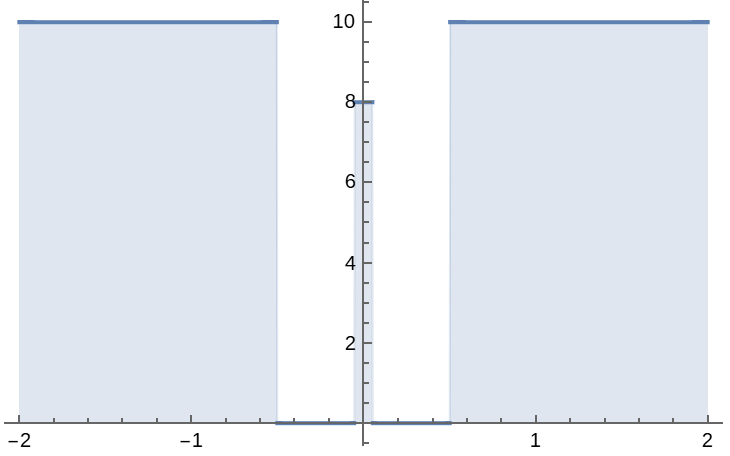
\includegraphics[width=\textwidth]{III3_taller.png}
        \caption{$h$ increased from $5V$ to $8V$}
        \label{fig:fig1}
    \end{subfigure}
    \hfill
    \begin{subfigure}[b]{0.45\textwidth}
        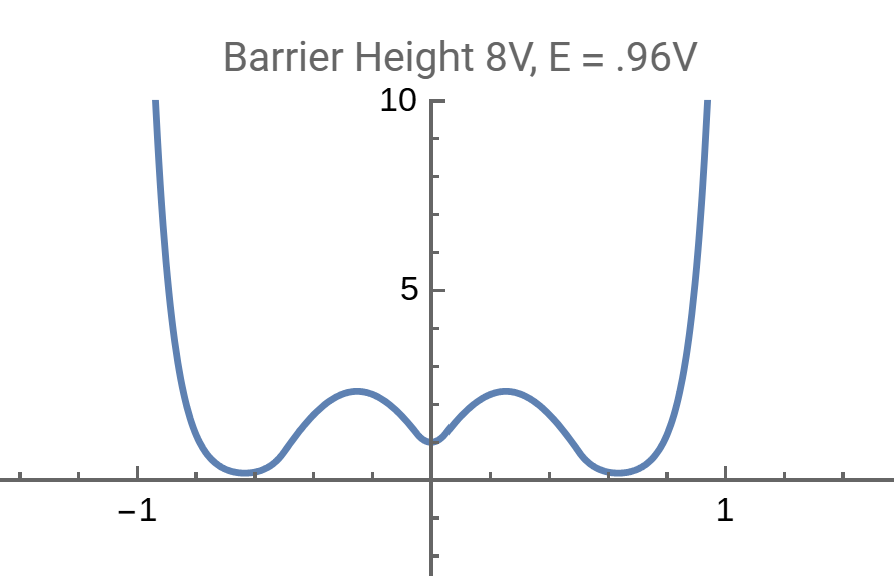
\includegraphics[width=\textwidth]{III3_tallerSol.png}
        \caption{Solution for the taller barrier}
        \label{fig:fig2}
    \end{subfigure}
    \
    \begin{subfigure}[b]{0.45\textwidth}
        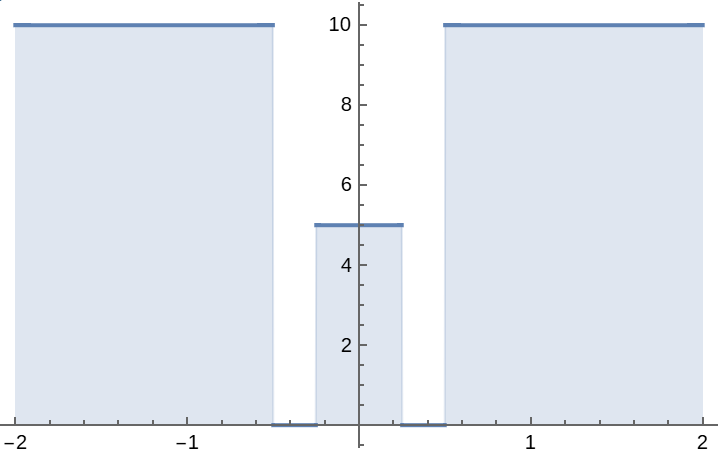
\includegraphics[width=\textwidth]{III3_wider.png}
        \caption{Wider barrier, $w = .5x_0$}
        \label{fig:fig3}
    \end{subfigure}
    \hfill
    \begin{subfigure}[b]{0.45\textwidth}
        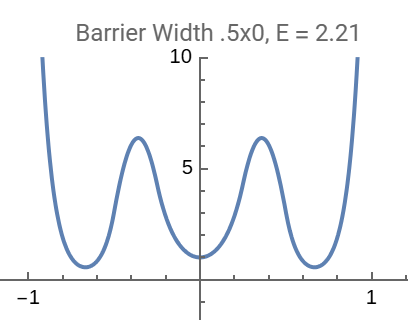
\includegraphics[width=\textwidth]{III3_widerSol.png}
        \caption{Solution for wider barrier}
        \label{fig:fig4}
    \end{subfigure}
    \label{fig:overall}
\end{figure}

We notice that the taller and the wider the barrier, 
the dimple of the first energy eigenstate gets bigger. 

\subsection{Limiting case}
As we increase the height of the well and the width, 
the energy of the first eigenvalue approaches that 
of an infinite square well. 


\end{document}